\documentclass[../main.tex]{subfiles}
\graphicspath{ {../img/} }


\begin{document}


	\chapter{Our implementation and design}

    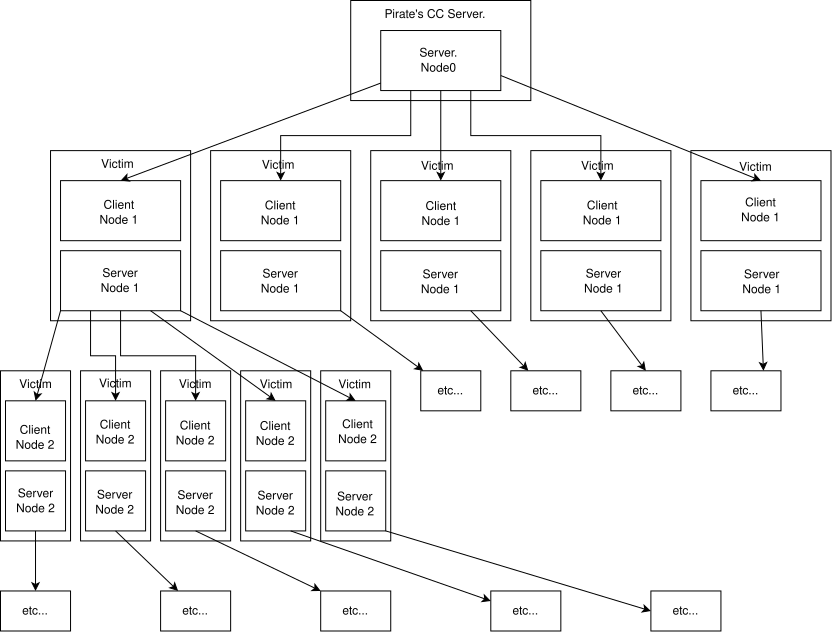
\includegraphics[width=450pt]{botnet.png}

    \vspace{10pt}

    \section{Things necessary for the project we had to either find or makes.}

    Our project had different parts.

    \begin{itemize}

        \item Making a sandbox environment while ensuring the worm does not escape.
        We used qemu and unshare to make an environnment that couldn't reach the external network.
        In the end it was unnecessary because we decided that for the demonstration the victim ip will be known before launch time, to prevent unexpected results in the final demo. 

        \item Finding an exploit to use.
        We needed the exploit to perform remote code execution, be easy to setup and use because the point of this project was not to create an intricate exploit, but rather to build a botnet.
        We spent hours looking for the perfect exploit and in the end we found a repository on github which performed in a way that we wanted.
        (https://github.com/opsxcq/
        exploit-CVE-2014-6271)
        Thanks to the work of opsxcq, we had an easy vulnerability to exploit.
        This vulnerability was CVE-2014-6271, known as Shellshock.
        In opsxcq's repository there was a docker image vulernable to Shellshock which was run by a simple command.
        There were two other vulnerabilities in his github that we were interested in but ultimately chose to not use: CVE-2016-10033 and CVE-2017-7494.
        There were both unsuitable for our application and would have required to much effort to get working. 
        We also considered log4j but decided to use an easier exploit to implement.

        \item Demonstrate the botnet.
        In order to demonstrate that the botnet worked we had to prove that the botnet has really taken control of several machine.
        To accomlish this we created a VM called vulnerableDOS. This VM would run wireshark and, once the botnet has taken control of the bots, receive and display the pings in the interace of wireshark.
        At first we wanted to make our botnet run an actual DDOS attack on the vulnerableDOS machine, but the purpose of the project was not to make it run a complex attack because our goal was just to prove that we have indeed taken control of the vulnerables machines. Because of this, we chose to simply ping the vulnerable DOS VM.

    \end{itemize}

    Of course, we also had to make the botnet itself 

    \vspace{10pt}

    \section{Botnet design}

    Designing and making the botnet was a real challenge. 
    The architecture of our botnet would consist of a server and a client. The server had three tasks. 
    Firstly it runs the exploit against the victim in a thread.
    Secondly, it runs a Command and Control server (CC), in another thread, to deliver it's order.
    The first order will always be to replicate the server on the victim, and the second one to ping the vulnerableDOS VM.
    Thirdly, the server runs a file sharing server (fs), so that every time the CC server ask the victim to download a file, the file can be downloaded.

    On the CC and the fs server, we implemented a TLS connection, using rustls. 
    The certificates used are self signed certificates, and every time the server is copied into the victim, openssl is used to generate the certificates.
    We were really lucky to find that openssl 1.0f was installed on the vulnerable image. 
    If the docker image was made two year ealier, openssl probably wouldn't have been installed, forcing us to abandon the idea of using encrypted connections.

    The goal of the client is to connect to the server, get its orders, and execute whatever the orders entail.

    The server reads TLS certificates from the conf folder, and the orders file that it transmits to the victim.
    It also creates files in the www directory eg.the list of ips that the next victim have to attack, a config file to easily generate new certificates, the exploit to run in order to run the client on the victim, and an installation script. In summary, the server permits the client to install whatever the servers serves and to replicate the server itself.

    \vspace{10pt}

    \section{Lab setup}

    To set up the lab environment we first made a VM, with the dinit init system on it, aswell as basic packages.
    We did this to be aware of all the programs running on the VM so that we didn't lose excessive time searching for bugs caused by clashes in the OS.
    We then made a VM to be the head of our botnet, 2 vulnerable vm and 1 more VM named vulnerableDOS.
    We called the first VM attacker, as it was going to be the initial aggresor in the demonstration.
    The two vulnerable VMs were called vulnerable1 and vulnerable2.
    These were going to be infected by the malware and added to the botnet.
    vulnerableDOS was going to be the vicitm of the botnet's ping attack.
    This means that our botnet project can be considered a success if we manage to make vulnerable1 and vulnerable2 ping vulnerableDOS.

    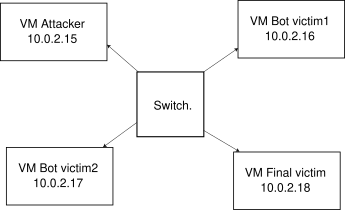
\includegraphics[width=450pt]{lab_env.png}


    \vspace{10pt}

    \section{Botnet communication}

    The following is the flow of the botnet's activity:
    Step one. 
    The server finds an potential target, within the demo, this target is specified.
    It runs a BASH script, called exploit.sh, which executes the exploit against the target.
    The exploit controls the victim in order to make the victim download and execute the client binary.
    In our case, the client is installed and run in `/tmp/botnet/`.

    Step two.
    The client requests the server for its first instruction, called order1.
    The server answers with the file and the client saves it in `/tmp/botnet/conf/`.

    Step three.
    The client reads the received order and every time it reachs a line begining with `download`, it requests the filesharing server for the respective file to download which is saved to `/tmp/botnet/downloaded/`.
    Everytime the client reaches a line begining with 'execute', it executes the file.

    Normally, only the file 'installation.sh' is executed at this stage.
    This script copies all the downloaded files from `/tmp/botnet/downloaded` to their respective folders.
    Now the server is run on the victim, which begins to look for other victims.

    Step four.
    Finally, once the victim runs its version of the server, it asks for its attack order from the CC server, which is called order2.
    Typically, an order2 file will ask the client to download and execute a BASH script.
    This BASH script will run the attack.
    In the case of the demo, it will only run `ping 10.0.2.18` for simplicity.

    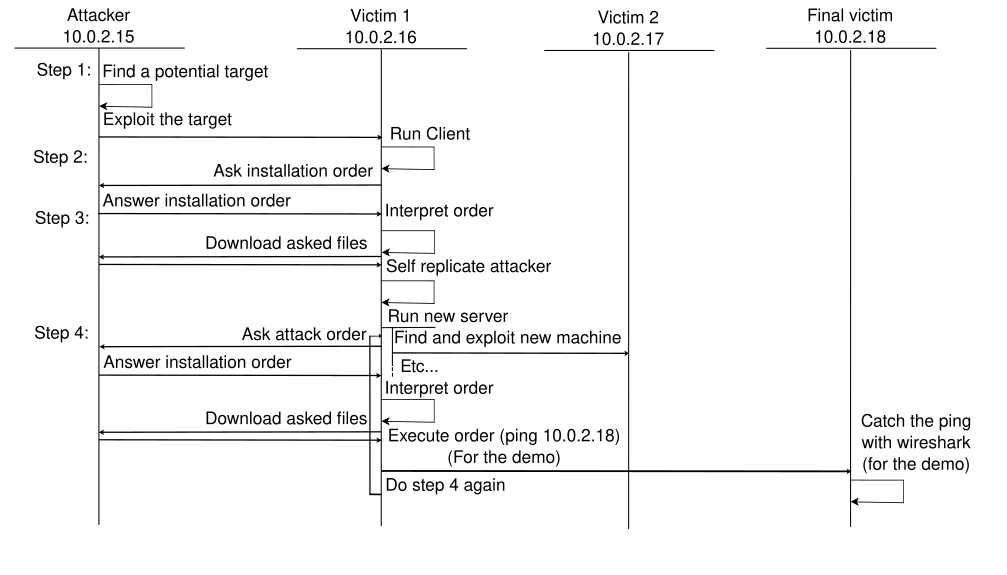
\includegraphics[width=450pt]{botnet_flow.png}

    Note that every time it receives an order, it will save it, and make it accessible to the server so that is can relay the orders to its child node, ie. the victim of the server that is being run.
    The same is true for every file that is downloaded.

    Having explained the thought process behind the design of the project, let us now look at the code.


\end{document}
